% !TeX program = xelatex
\documentclass[10pt,a4paper]{ctexart} % 设置文章类型，正文字号与纸张大小

% 页面与正文常用宏包
\usepackage[margin=2cm]{geometry} % 设置页面四周页边距
\usepackage{graphicx}             % 插入图片
\usepackage{amsmath}              % 提供cases、aligned等数学公式环境
\usepackage{amssymb}              % 提供\therefore等扩展数学符号
\usepackage{booktabs}             % 提供\toprule、\midrule、\bottomrule三线表命令
\usepackage{float}                % 提供[H]固定图片、表格位置
\usepackage{subcaption}           % 提供subfigure子图环境及子图标题
\usepackage{wrapfig}              % 提供wrapfigure图文环绕环境
\usepackage{fancyhdr}             % 自定义页眉和页脚
\usepackage{hyperref}             % 生成超链接

% 页眉页脚
\pagestyle{fancy}                  % 启用fancyhdr定义的页面样式
\fancyhf{}                         % 清空默认页眉和页脚
\fancyfoot[C]{\thepage}            % 在页脚中央显示页码
\renewcommand{\headrulewidth}{0pt} % 隐藏页眉横线
\renewcommand{\footrulewidth}{0pt} % 隐藏页脚横线

% 超链接
\hypersetup{
  colorlinks=true,                % 使用彩色文字链接，而非带边框的链接
  linkcolor=red,                 % 目录、公式及图表交叉引用的颜色
  filecolor=cyan,                 % 本地文件链接的颜色
  urlcolor=blue,                  % 网址链接的颜色
  pdftitle={示波器的使用+组装整流器预习报告},     % 写入PDF文档属性的标题
  bookmarksnumbered=true          % PDF书签显示章节编号
}

% 定义字号命令
\newcommand{\chuhao}{\fontsize{42pt}{63pt}\selectfont}
\newcommand{\xiaochu}{\fontsize{36pt}{54pt}\selectfont}
\newcommand{\yihao}{\fontsize{26pt}{39pt}\selectfont}
\newcommand{\xiaoyi}{\fontsize{24pt}{36pt}\selectfont}
\newcommand{\erhao}{\fontsize{22pt}{33pt}\selectfont}
\newcommand{\xiaoer}{\fontsize{18pt}{27pt}\selectfont}
\newcommand{\sanhao}{\fontsize{16pt}{24pt}\selectfont}
\newcommand{\xiaosan}{\fontsize{15pt}{22.5pt}\selectfont}
\newcommand{\sihao}{\fontsize{14pt}{21pt}\selectfont}
\newcommand{\xiaosi}{\fontsize{12pt}{18pt}\selectfont}
\newcommand{\wuhao}{\fontsize{10.5pt}{15.75pt}\selectfont}
\newcommand{\xiaowu}{\fontsize{9pt}{13.5pt}\selectfont}

% 章节格式
\ctexset{
  section={
    format={\CJKfontspec[AutoFakeBold=2.5]{KaiTi}\sanhao\bfseries}, % 一级标题使用三号加粗楷体
    name={,、},                                                    % 在中文章节序号后添加顿号
    number=\chinese{section},                                      % 一级标题编号使用“一、二、三”形式
    aftername={}                                                   % 取消编号与标题文字之间的空格
  },
  subsection={
    format={\CJKfontspec[AutoFakeBold=2.5]{KaiTi}\sihao\bfseries}, % 二级标题使用四号加粗楷体
  },
  subsubsection={
    format={\CJKfontspec[AutoFakeBold=2.5]{KaiTi}\xiaosi\bfseries}, % 三级标题使用小四加粗楷体
  }
}

\begin{document}

% 封面
\thispagestyle{fancy} % 封面保留底部居中的页码
\fancyfoot[C]{\thepage}
\begin{center}
  \CJKfontspec[AutoFakeBold=2.5]{KaiTi}\bfseries % 封面中文使用楷体并人工加粗，西文同时加粗
  \vspace*{2.0cm}
  \xiaochu 
    物理实验预习报告

  \vspace{3.8cm}
  \begin{minipage}{10.0cm}
    \sanhao
    \makebox[2.6cm][l]{实验名称：}
    \underline{\makebox[7.0cm][c]{示波器的使用+组装整流器}}\par\vspace{12pt}

    \makebox[2.6cm][l]{指导老师：}
    \underline{\makebox[7.0cm][c]{居乐乐}}\par\vspace{12pt}
  \end{minipage}

  \vspace{3.8cm}
  \begin{minipage}{10.0cm}
    \sihao
    \makebox[1.4cm][l]{班级：}
    \underline{\makebox[8.0cm][c]{}}\par\vspace{10pt}

    \makebox[1.4cm][l]{姓名：}
    \underline{\makebox[8.0cm][c]{IllusoryRain}}\par\vspace{10pt}

    \makebox[1.4cm][l]{学号：}
    \underline{\makebox[8.0cm][c]{}}
  \end{minipage}

  \vspace{1.8cm}
  \sihao
    实验日期：
    \underline{\makebox[0.7cm][c]{2026}}年
    \underline{\makebox[0.7cm][c]{10}}月
    \underline{\makebox[1.4cm][c]{10/14}}日
    星期\underline{\makebox[1.4cm][c]{六/三}}上午

  \vspace{0.7cm}
  \sihao 
    浙江大学物理实验教学中心
\end{center}

\newpage
\xiaosi\songti\mdseries % 后续正文统一使用小四宋体

\section{预习报告（10分）}

  \subsection{实验综述（5分）}

    \subsubsection{示波器的使用}
    示波器的原理：示波器能将振荡信号以波形（正弦波、方波、锯齿波）显示在荧光屏上。
    它由示波管、放大器（包括X轴放大和Y轴放大）、扫描与触发同步系统和电源四个基本部分组成。

    李萨如图形是两个相互垂直的简谐振动叠加形成的轨迹。
    在X--Y模式下，将两路正弦信号分别接入CH1（X轴）和CH2（Y轴），
    当频率比为稳定的整数比时，可观察到稳定图形，并据此测量未知频率。

    信号频率和该轴上交点的数量成反比：
    \[
      \frac{f_y}{f_x}=\frac{T_x}{T_y}=\frac{N_x}{N_y},
      \qquad f_y=\frac{N_x}{N_y}f_x
    \]
    其中$N_x$、$N_y$分别为水平、竖直参考线的交点数。
    已知CH1（X轴）信号频率，即可测量CH2（Y轴）信号的频率；同频时也可测量相位差。

    \begin{figure}[H]
      \centering
      \begin{minipage}[c]{0.48\textwidth}
        \centering
        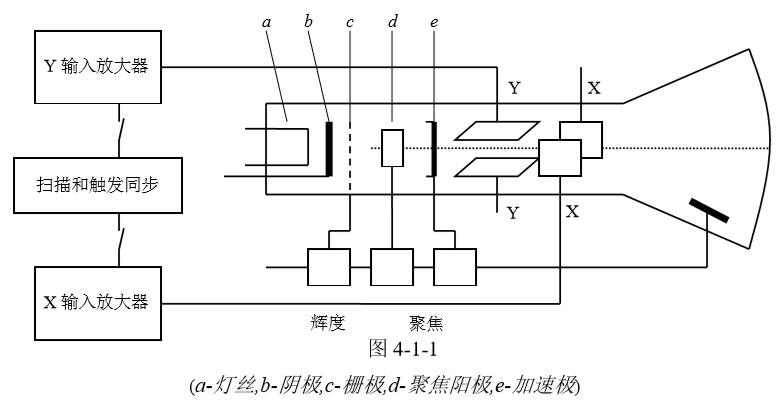
\includegraphics[width=0.95\textwidth]{figures/图1.png}
        \caption{示波器的基本结构}
      \end{minipage}
      \begin{minipage}[c]{0.48\textwidth}
        \centering
        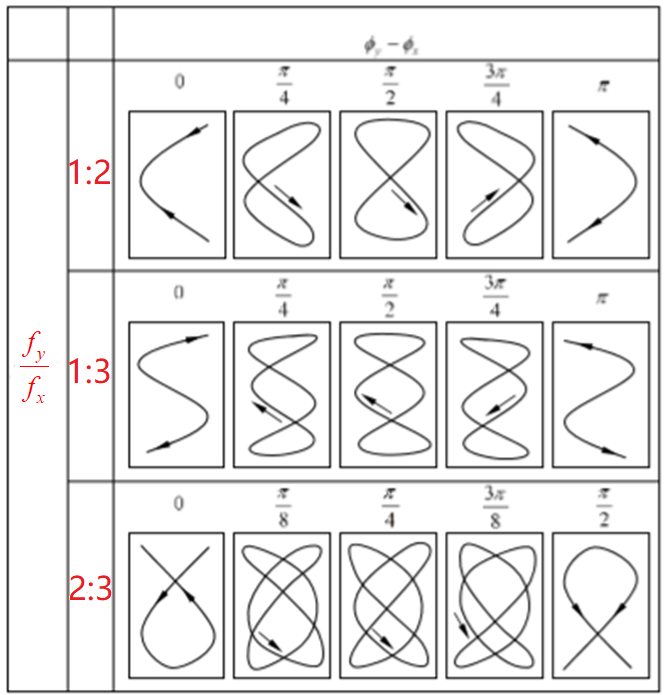
\includegraphics[width=0.8\textwidth]{figures/图2.png}
        \caption{不同频率比、相位差下的李萨如图形}
      \end{minipage}
    \end{figure}

    本实验包括以下三项内容：
    \begin{enumerate}
      \item 李萨如图测量未知频率：将已知频率信号接入X轴、未知信号接入Y轴，微调已知频率，
      待图形稳定后，记录交点数，按上述频率关系计算未知频率。

      \item 二极管导通电压测量：双通道同时观察二极管电路的输入、输出波形，
      用光标法或直读法读取电压，由输入、输出正峰值之差估算导通电压。
      
      \item RC电路相位差测量：双通道同时观察输入、输出波形，测量周期及对应特征点的时间差，
      根据时间差与周期的比值求出相位差，并判断输出信号的超前或滞后。
    \end{enumerate}

    \subsubsection{组装整流器}
    单相半波整流电路：
    \begin{itemize}
      \item 输出电压平均值：
      \[
        \overline{U}_0
        = \frac{1}{2\pi} \int_0^\pi
          \left(\sqrt{2}U_2\right)\sin(\omega t)\,\mathrm{d}(\omega t)
        = \frac{\sqrt{2}}{\pi}U_2
        = 0.45U_2
      \]

      \item 二极管承受最大反向电压：$\sqrt{2}U_2$

      \item 缺点：输出电压脉动大、效率低、二极管承受的反向电压大
    \end{itemize}

    \begin{figure}[H]
      \centering
      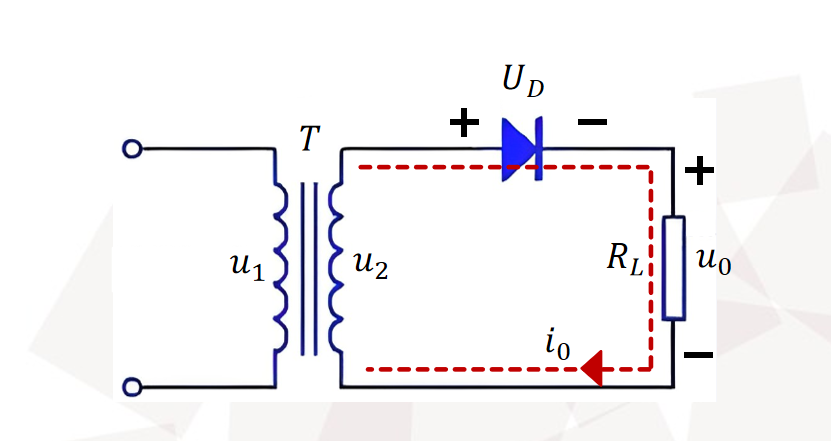
\includegraphics[width=0.4\textwidth]{figures/图3.png}
      \caption{单相半波整流电路}
    \end{figure}
    
    单相全波整流电路：
    \begin{itemize}
    \item 输出电压平均值：
    \[
        \overline{U}_0
        = \frac{1}{\pi}\int_{0}^{\pi}
        \left(\sqrt{2}U_2\right)\sin(\omega t)\,\mathrm{d}(\omega t)
        = \frac{2\sqrt{2}}{\pi}U_2
        = 0.9U_2
    \]

    \item 二极管承受最大反向电压：$2\sqrt{2}U_2$

    \item 缺点：电路结构复杂，需要中央抽头；二极管承受反向电压大
    \end{itemize}

    \begin{figure}[H]
      \centering
      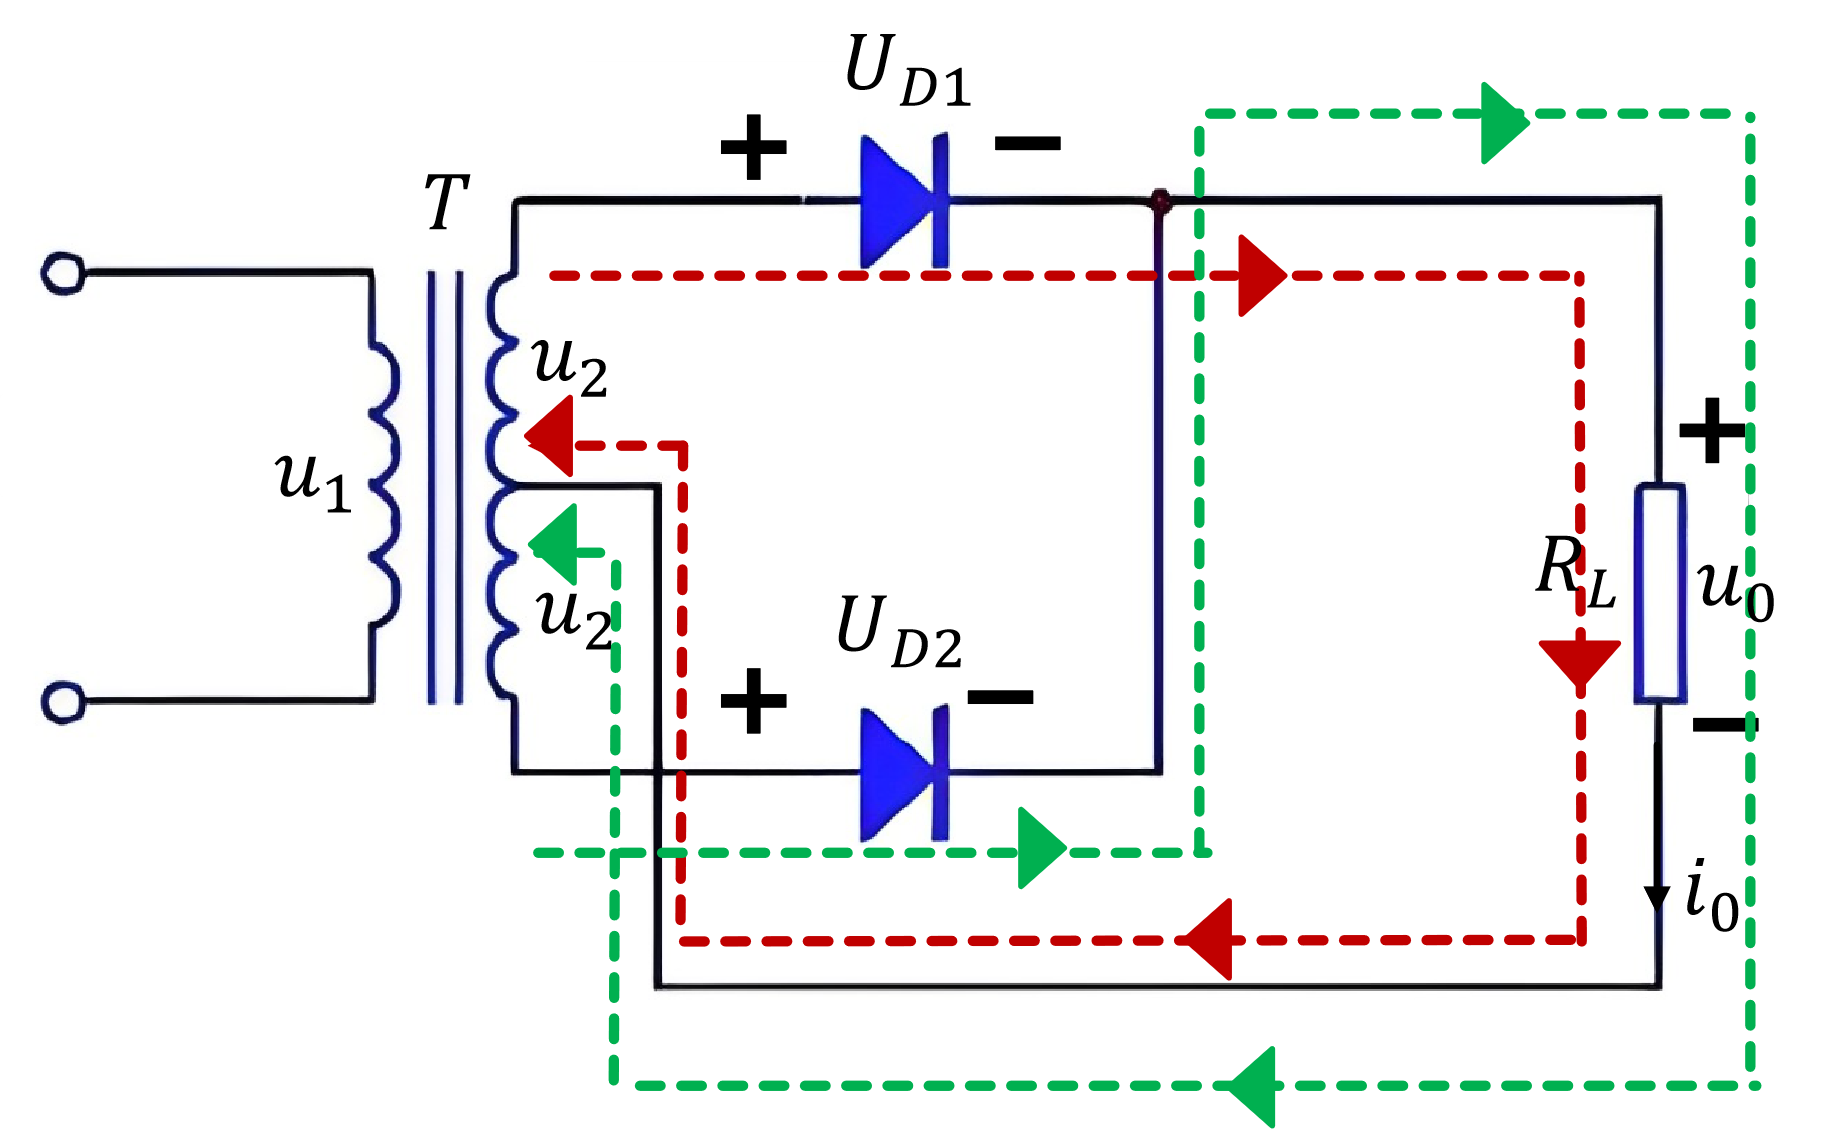
\includegraphics[width=0.4\textwidth]{figures/图4.png}
      \caption{单相全波整流电路}
    \end{figure}

    \newpage
    
    单相桥式整流电路：
    \begin{itemize}
    \item 输出电压平均值：
    \[
        \overline{U}_0
        = \frac{1}{\pi}\int_{0}^{\pi}
        \left(\sqrt{2}U_2\right)\sin(\omega t)\,\mathrm{d}(\omega t)
        = \frac{2\sqrt{2}}{\pi}U_2
        = 0.9U_2
    \]

    \item 二极管承受最大反向电压：$2\sqrt{2}U_2$

    \item 缺点：电路结构复杂，需要中央抽头；二极管承受反向电压大
    \end{itemize}

    \begin{figure}[H]
      \centering
      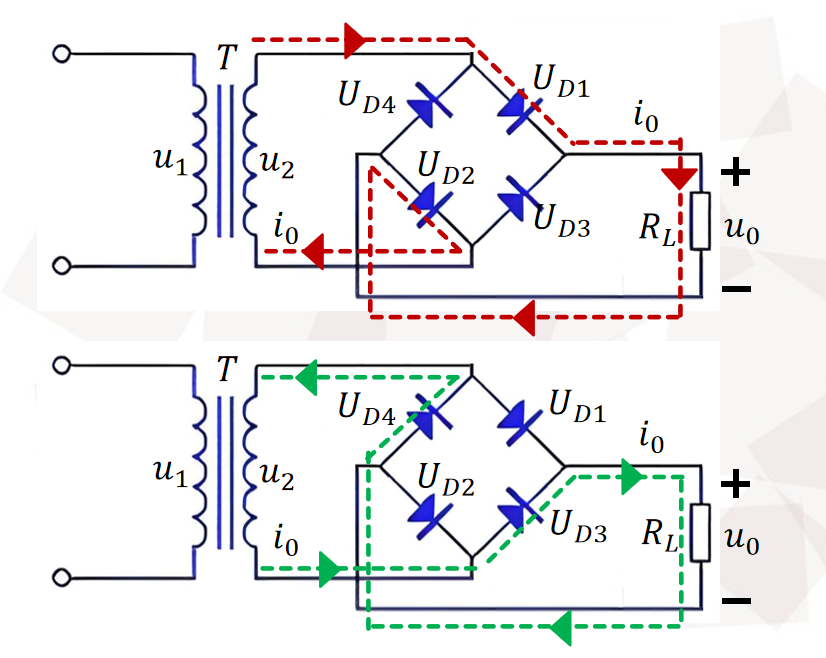
\includegraphics[width=0.4\textwidth]{figures/图5.png}
      \caption{单相桥式整流电路}
    \end{figure}

    滤波电路：
    \begin{figure}[H]
      \centering
      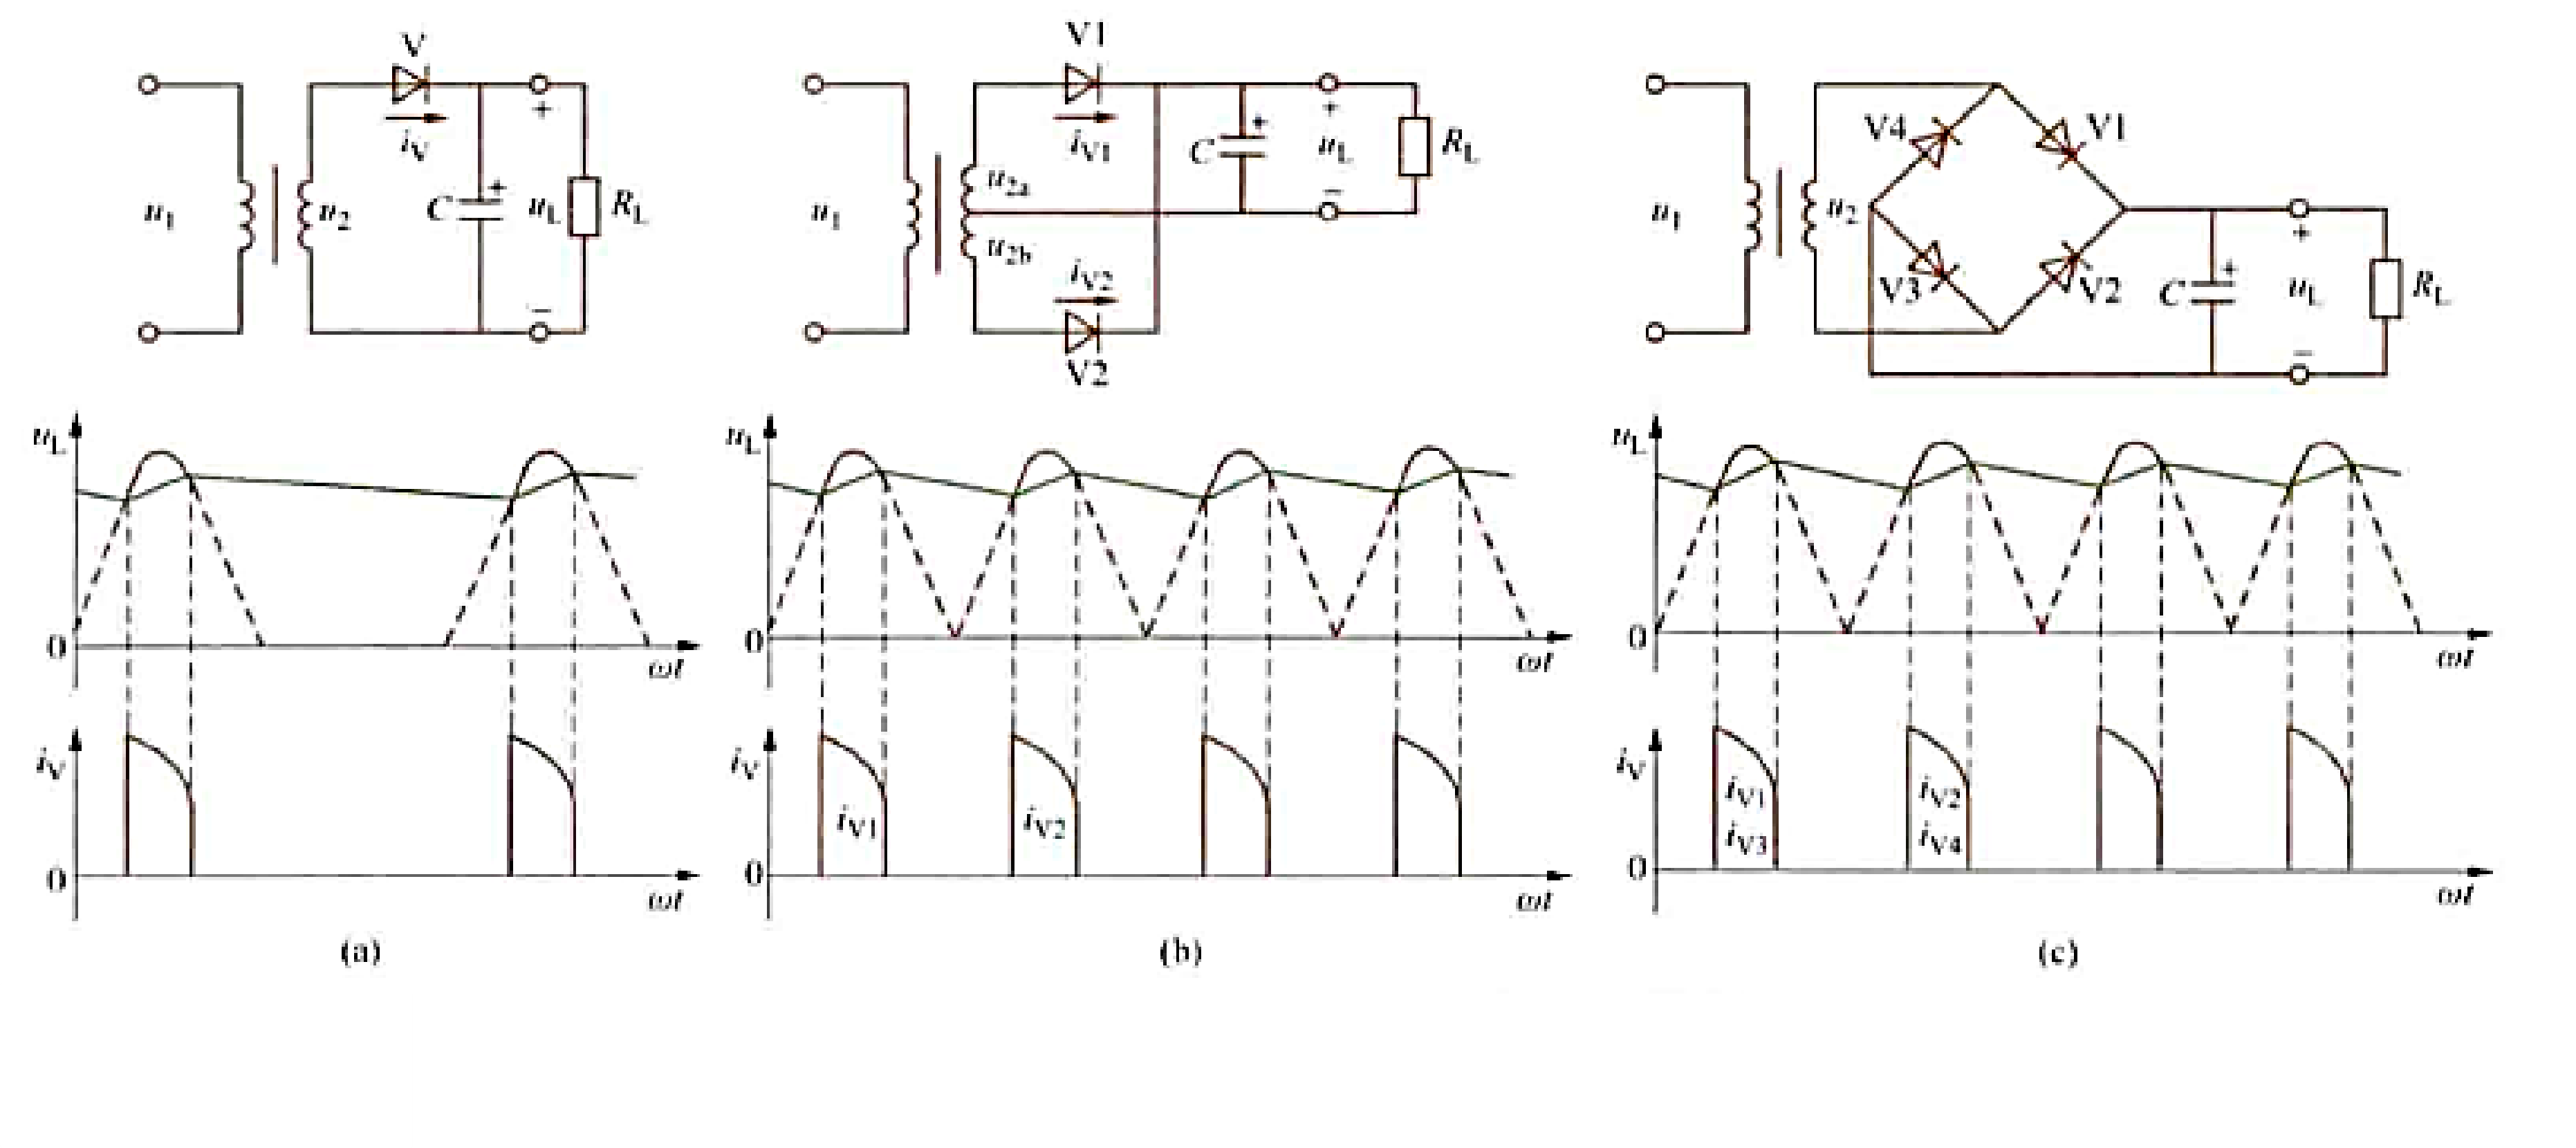
\includegraphics[width=0.6\textwidth]{figures/图6.png}
      \caption{滤波电路}
    \end{figure}

    实验包括以下两部分内容：

    组装整流电路：
    \begin{enumerate}
    \item 搭建单相半波整流电路、全波整流电路以及桥式整流电路。（示波器耦合模式：直流输入）观察输入波形、输出波形和二极管的反向电压波形，在表格中描绘波形。

    \item 使用示波器测量三种整流电路的以下参数，并在实验数据记录表格中记录：
      \begin{itemize}
        \item 输入信号的有效值$U_2$。
        \item 整流电路输出信号的有效值$U_0$和平均值$\overline{U}_0$。
        \item 整流电路中某个二极管的反向电压峰值$U_{\mathrm{Rmax}}$。
      \end{itemize}

    \item 计算无滤波器情况下，输出电压的平均值$\overline{U}_0$与公式所得的理论值之间的相对误差。
    \end{enumerate}
    
    观察RC滤波的效果：
    
    对于三种整流电路，分别添加47$\mu$F和470$\mu$F两种不同电容。观察RC滤波后的输出波形变化。
    比较不同电容值的滤波效果差异，并完成表格。
    
  \subsection{实验重点（3分）}
  
    \subsubsection{示波器的使用}
    \begin{enumerate}
      \item 从物理学角度了解示波器的结构和工作原理，了解示波器的扫描原理。
      \item 熟悉示波器面板旋钮的功能，掌握示波器的调节和使用方法。
      \item 学习用示波器观察信号波形，并测量其幅度大小、周期（或频率）、相位。
      \item 掌握用李萨如图形测量正弦信号频率的原理和方法。
    \end{enumerate}

    \subsubsection{组装整流器}
    \begin{enumerate}
      \item 了解整流电路与滤波电路的功能。
      \item 完成三种整流电路以及滤波电路的设计与组装。
      \item 熟悉掌握数字示波器的使用，了解一些常用电子元件的使用方法。
    \end{enumerate}

  \subsection{实验难点（2分）}

    \subsubsection{示波器的使用}
    \begin{enumerate}
      \item 调节时基与触发使波形稳定，正确判读李萨如图形的交点数与频率比。
      \item 准确读取输入、输出正峰值，利用其差值估算二极管导通电压。
      \item 测量RC电路输入、输出的周期和时间差，计算相位差并判断超前或滞后。
    \end{enumerate}

    \subsubsection{组装整流器}
    \begin{enumerate}
      \item 正确连接半波、全波和桥式整流电路，注意二极管方向及滤波电容极性。
      \item 区分有效值、平均值与峰值，准确测量整流电路各项电压参数。
      \item 比较两种电容的滤波效果，并计算无滤波时输出平均电压与理论值的相对误差。
    \end{enumerate}

\vspace*{\fill} % 使下面内容在页面底部显示
\noindent
\begin{minipage}{\textwidth}
  注意事项：

  \begingroup
    \setlength{\leftskip}{2em} % 1--4整体向右缩进两个汉字宽度
    1. 用PDF格式上传“实验报告”，文件名：学生姓名+学号+实验名称+周次。

    2. “实验报告”必须递交在“学在浙大”本课程内对应实验项目的“作业”模块内。

    3. “实验报告”成绩必须在“浙江大学物理实验教学中心网站”-“选课系统”内查询。

    4. 教学评价必须在“浙江大学物理实验教学中心网站”-“选课系统”内进行，学生必须进行教学评价，才能看到实验报告成绩，教学评价须在本次实验结束之后3天内进行。\par
  \endgroup

  \begin{center}
    {\CJKfontspec[AutoFakeBold=2.5]{SimSun}\bfseries 浙江大学物理实验教学中心制}
  \end{center}
\end{minipage}

\end{document}


